\documentclass[11pt]{article}
\usepackage{xeCJK}
\usepackage[a4paper, margin=1.4in]{geometry}
\usepackage{fancyhdr}
\usepackage{amsmath}
\usepackage{amssymb}
\usepackage{graphicx}
\usepackage[most]{tcolorbox}
\usepackage{framed} 
\usepackage{tikz}
\usepackage{hyperref}

\linespread{1.25}
\setlength\parindent{0pt}

\usetikzlibrary{matrix,chains,positioning,decorations.pathreplacing,arrows}

\title{%
  \LARGE
  \textbf{COMP90086 Computer Vision \\
  \large Week 4
  \\
  CNN}}
\author{ Lecture Notes summarized by Neo }
\date{Semester 2 2021}

\pagestyle{fancy}
\fancyhf{}
\rhead{COMP90086 Computer Vision}
\lhead{Lecture Notes}
\rfoot{Page \thepage}

\begin{document}

\maketitle


\section{Artificial Neural Network}
\subsection{Definition}
人工神经网络\footnote{https://en.wikipedia.org/wiki/Artificial\_neural\_network}(英語:Artificial Neural Network,ANN),简称神经网络(Neural Network,NN)或類神經網絡,在机器学习和认知科学领域,是一种模仿生物神经网络(动物的中樞神經系統,特别是大脑)的结构和功能的数学模型或计算模型,用于对函数进行估计或近似。神经网络由大量的人工神经元联结进行计算。大多数情况下人工神经网络能在外界信息的基础上改变内部结构,是一种自适应系统,通俗地讲就是具备学习功能。现代神经网络是一种非线性统计性数据建模工具,神经网络通常是通过一个基于数学统计学类型的学习方法(Learning Method)得以优化,所以也是数学统计学方法的一种实际应用,通过统计学的标准数学方法我们能够得到大量的可以用函数来表达的局部结构空间,另一方面在人工智能学的人工感知领域,我们通过数学统计学的应用可以来做人工感知方面的决定问题,这种方法比起正式的逻辑学推理演算更具有优势。
\begin{framed}
  \begin{center}
    ANN是神经网络的一个统称,有不同种类,例如MLP和CNN等等。
  \end{center}
\end{framed}
\subsection{Type}
\begin{itemize}
  \item Multilayer Perceptron (MLP)
  \item Convolutional Neural Network (CNN)
  \item ...
\end{itemize}


\section{Multilayer Perceptron (MLP) 多层感知器}
\subsection{Perceptron}
Perceptron is a \textbf{single layer neural network} and a multi-layer perceptron is called Neural Networks.\\
感知机\footnote{https://en.wikipedia.org/wiki/Perceptron}是生物神经细胞的简单抽象。神经细胞结构大致可分为:树突、突触、细胞体及轴突。单个神经细胞可被视为一种只有两种状态的机器——激动时为『是』,而未激动时为『否』。神经细胞的状态取决于从其它的神经细胞收到的输入信号量,及突触的强度(抑制或加强)。当信号量总和超过了某个阈值时,细胞体就会激动,产生电脉冲。电脉冲沿着轴突并通过突触传递到其它神经元。为了模拟神经细胞行为,与之对应的感知机基础概念被提出,如权量(突触)、偏置(阈值)及激活函数(细胞体)。

在人工神经网络领域中,感知机也被指为单层的人工神经网络,以区别于较复杂的多层感知机(Multilayer Perceptron)。作为一种线性分类器,(单层)感知机可说是最简单的前向人工神经网络形式。尽管结构简单,感知机能够学习并解决相当复杂的问题。感知机主要的本质缺陷是它不能处理线性不可分问题。
\begin{center}

  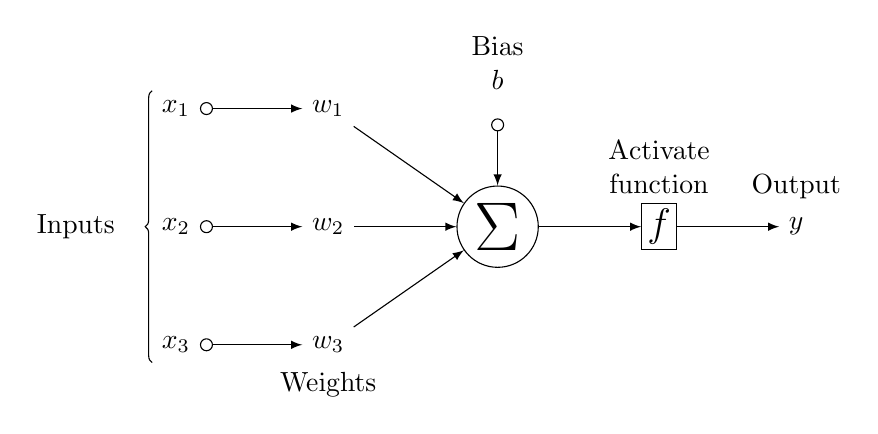
\begin{tikzpicture}[
      init/.style={
          draw,
          circle,
          inner sep=2pt,
          font=\Huge,
          join = by -latex
        },
      squa/.style={
          draw,
          inner sep=2pt,
          font=\Large,
          join = by -latex
        },
      start chain=2,node distance=13mm
    ]
    \node[on chain=2]
    (x2) {$x_2$};
    \node[on chain=2,join=by o-latex]
    {$w_2$};
    \node[on chain=2,init] (sigma)
    {$\displaystyle\Sigma$};
    \node[on chain=2,squa,label=above:{\parbox{2cm}{\centering Activate \\ function}}]
    {$f$};
    \node[on chain=2,label=above:Output,join=by -latex]
    {$y$};
    \begin{scope}[start chain=1]
      \node[on chain=1] at (0,1.5cm)
      (x1) {$x_1$};
      \node[on chain=1,join=by o-latex]
      (w1) {$w_1$};
    \end{scope}
    \begin{scope}[start chain=3]
      \node[on chain=3] at (0,-1.5cm)
      (x3) {$x_3$};
      \node[on chain=3,label=below:Weights,join=by o-latex]
      (w3) {$w_3$};
    \end{scope}
    \node[label=above:\parbox{2cm}{\centering Bias \\ $b$}] at (sigma|-w1) (b) {};

    \draw[-latex] (w1) -- (sigma);
    \draw[-latex] (w3) -- (sigma);
    \draw[o-latex] (b) -- (sigma);

    \draw[decorate,decoration={brace,mirror}] (x1.north west) -- node[left=10pt] {Inputs} (x3.south west);
  \end{tikzpicture}

\end{center}

\begin{itemize}
  \item Weights shows the strength of the particular node.
  \item The bias value allows you to shift the activation function curve up or down.
  \item The activation functions are used to map the input between the required values like (0, 1) or (-1, 1).
\end{itemize}

\begin{framed}
  \begin{center}
    Perceptron is usually used to classify the data into two parts. Therefore, it is also known as a \textbf{Linear Binary Classifier}.
  \end{center}
\end{framed}

\subsection{Multilayer Perceptron}
A multilayer perceptron (MLP) is a class of feedforward artificial neural network (ANN). The term MLP is used ambiguously, sometimes loosely to mean any feedforward ANN, sometimes strictly to refer to networks composed of multiple layers of perceptrons (with threshold activation).\\
多层感知器\footnote{https://en.wikipedia.org/wiki/Multilayer\_perceptron}(Multilayer Perceptron, 缩写MLP)是一种前向结构的人工神经网络,映射一组输入向量到一组输出向量。MLP可以被看作是一个有向图,由多个的节点层所组成,每一层都全连接到下一层。除了输入节点,每个节点都是一个带有非线性激活函数的神经元(或称处理单元)。一种被称为反向传播算法的监督学习方法常被用来训练MLP。MLP是感知器的推广,克服了感知器不能对线性不可分数据进行识别的弱点。
\begin{center}

  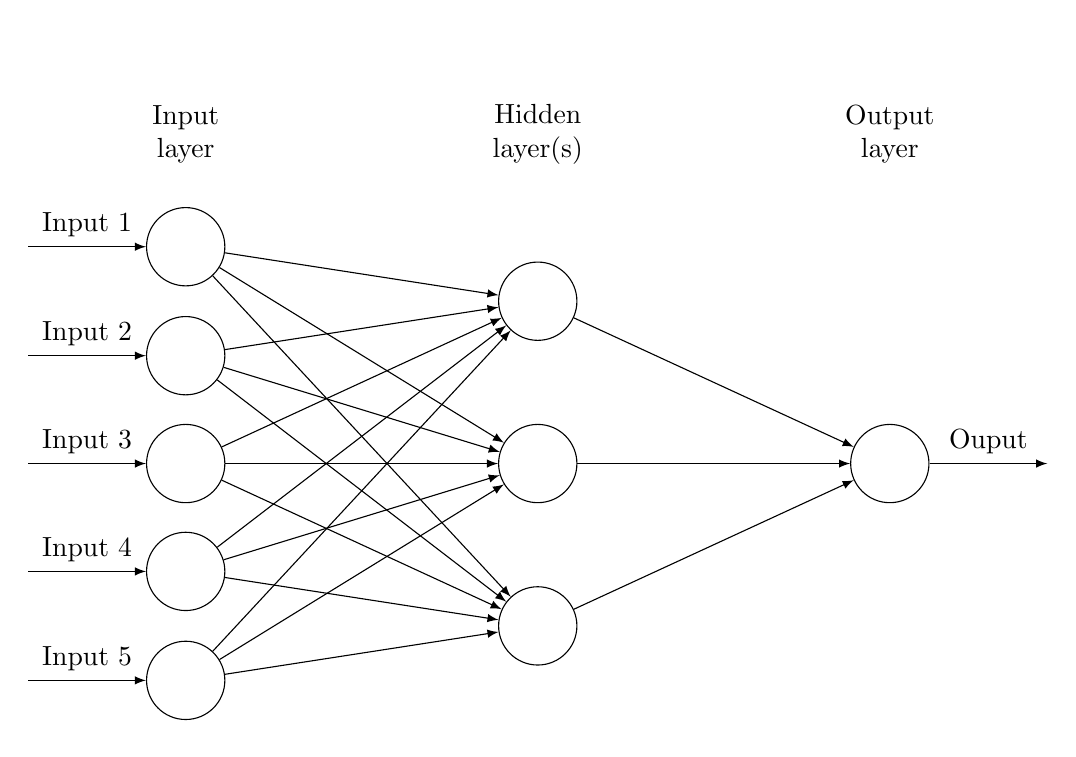
\begin{tikzpicture}[
      plain/.style={
          draw=none,
          fill=none,
        },
      net/.style={
          matrix of nodes,
          nodes={
              draw,
              circle,
              inner sep=10pt
            },
          nodes in empty cells,
          column sep=2cm,
          row sep=-9pt
        },
      >=latex
    ]
    \matrix[net] (mat)
    {
    |[plain]| \parbox{1.3cm}{\centering Input\\layer} & |[plain]| \parbox{1.3cm}{\centering Hidden\\layer(s)} & |[plain]| \parbox{1.3cm}{\centering Output\\layer} \\
    & |[plain]| \\
    |[plain]| & \\
    & |[plain]| \\
    |[plain]| & |[plain]| \\
    & & \\
    |[plain]| & |[plain]| \\
    & |[plain]| \\
    |[plain]| & \\
    & |[plain]| \\    };
    \foreach \ai [count=\mi ]in {2,4,...,10}
    \draw[<-] (mat-\ai-1) -- node[above] {Input \mi} +(-2cm,0);
    \foreach \ai in {2,4,...,10}
      {\foreach \aii in {3,6,9}
        \draw[->] (mat-\ai-1) -- (mat-\aii-2);
      }
    \foreach \ai in {3,6,9}
    \draw[->] (mat-\ai-2) -- (mat-6-3);
    \draw[->] (mat-6-3) -- node[above] {Ouput} +(2cm,0);
  \end{tikzpicture}

\end{center}

\begin{framed}
  \begin{center}
    MLP通常被视为``最经典的"人工神经网络。
  \end{center}
\end{framed}


\subsection{Problem}
MLP is now deemed insufficient for modern advanced computer vision tasks. Has the characteristic of \textbf{fully connected layers}, where each perceptron is connected with every other perceptron. Disadvantage is that the number of total parameters can grow to very high (number of perceptron in layer 1 multiplied by \# of p in layer 2 multiplied by \# of p in layer 3...). This is inefficient because there is redundancy in such high dimensions. Another disadvantage is that it disregards spatial information. It takes flattened vectors as inputs. (input图像会被展平成1d-vector导致图像物体位置无法体现。)


\section{Convolutional Neural Network (CNN) 卷积神经网络}

\subsection{Convolution 卷积 recap }
\begin{framed}
  \begin{center}
    The ``convolution" operation  in CNN is actually ``correlation" operation, i.e., the filter is not flipped before applying to the input. The difference between convolution and correlation (flip the filter or not) does not affect the performance of the algorithm. During training of CNN, the filter will adjust weights that are best suited for the correlation operation, so the flip is omitted.
  \end{center}
\end{framed}
\begin{figure}[hbt!]
  \centering
  \includegraphics[width=0.8\textwidth]{assets/cnn.png}
\end{figure}


\subsection{Motivation}
卷积可以用来探测图片与Kernel的相似程度,(通过把Kernel定义成不同的组合),所以我们可以使用很多个Kernel分别代表不同的``图像特征"与原图像做卷积。\\

图中的输入图像是(8,8,3),filter有4个,大小均为(3,3,3),得到的输出为(6,6,4)。(每一个Kernel与原图像三个RGB频道做卷积得到其中一层输出。)

\begin{figure}[hbt!]
  \includegraphics[width=\textwidth]{assets/cnn2.png}
  \centering
\end{figure}



\subsection{Stride 步长}
每两步卷积操作的距离,默认为1 (Kernel一格一格地挪)。Stride为2时如下图所示:

\begin{figure}[hbt!]
  \centering
  \includegraphics[width=0.75\textwidth]{assets/stride.png}
\end{figure}

\begin{itemize}
  \item No padding: output\_size = ceiling((input\_size-kernel\_size+1)/stride)
  \item With padding: output\_size = ceiling(input\_size/stride)
\end{itemize}


\subsection{Padding 填白}
由于经过卷积操作图像会变小,需要通过填白先使原图变大再做卷积,具体方式可详见Week2笔记。在使用代码框架时我们把``让卷积之后的大小不变"的padding方式,称为 ``Same"方式, 把不经过任何填白的,称为 ``Valid"方式。


\subsection{Pooling 池化}
为了提取一定区域的主要特征,并减少参数数量,防止模型过拟合。不需要考虑Kernel。
\begin{itemize}
  \item Max-Pooling\\
        取Kernel大小区域中的最大值,示例见下图。可以最大化提取区域特征。
  \item Average-Pooling\\
        取Kernel大小区域中的平均值
  \item ...
\end{itemize}

\begin{figure}[hbt!]
  \centering
  \includegraphics[width=0.8\textwidth]{assets/maxp.png}
\end{figure}


\section{CNN Layers}
部分笔记来自知乎@蝈蝈\footnote{https://zhuanlan.zhihu.com/p/42559190}
\subsection{Convolutional Layer 卷积层}
由Filters和Activate Function构成。 一般要设置的参数包括filters的数量、大小、步长,以及padding。

\subsection{Pooling Layer 池化层}
这里里面没有参数需要我们学习,因为这里里面的参数都是我们设置好了,要么是Maxpooling,要么是Averagepooling。 需要指定的超参数,包括是Max还是average,窗口大小以及步长。 通常,我们使用的比较多的是Maxpooling,而且一般取大小为(2,2)步长为2的filter,这样,经过pooling之后,输入的长宽都会减半,channels不变。

\subsection{Fully-Connected Layer 全连接层}
发生在\textbf{一次或数次}卷积层和池化层之后: 我们最后会先将多维的数据进行``扁平化",也就是把 (height,width,channel)的数据压缩成长度为 height × width × channel 的一维数组,然后再与FC层连接,这之后就跟普通的神经网络无异了。

\subsection{Visualization}
\begin{figure}[hbt!]
  \centering
  \includegraphics[width=\textwidth]{assets/layers.jpeg}
\end{figure}


\section{Separable Convolutions}
介绍两种如何把一个kernel分成两个kernel连续卷积的方法,具体的数学推导请详见Lecture Slides...
\subsection{Spatial Separable Convolutions}
一些Kernel可以分成两个1D矩阵相乘,如:
\begin{figure}[hbt!]
  \centering
  \includegraphics[width=0.8\textwidth]{assets/sep1.png}
\end{figure}
这样就可以对一个图像进行两次1D Filter的卷积,可以有效减少计算复杂度,提高训练速度。
\begin{figure}[hbt!]
  \centering
  \includegraphics[width=\textwidth]{assets/sep2.png}
\end{figure}
\begin{framed}
  \begin{center}
    之前提到的Sobel Filter用来探测边界就是利用了Spatial Seperable Convolutions的思想。
  \end{center}
\end{framed}

\begin{framed}
  \begin{center}
    问题: 不是所有的Kernel Matrix都可以分成两个Matrix相乘的形式。
  \end{center}
\end{framed}


\subsection{Depthwise Seperable Convolutions}
讲Kernel分为两个部分分别对原图像做Depth-wise Convolution和Point-wise Convolution。要注意不同步骤之间的维度转化,可见图:
\begin{figure}[hbt!]
  \centering
  \includegraphics[width=\textwidth]{assets/depth.png}
\end{figure}


\newpage
\section{Train CNN 训练模型}
\subsection{Gradient Descent 梯度下降}
...一些数学公式和算法,详见Lecture Slides,一般会使用第三方库直接操作...


\section{CNN Visualization (推荐)}
https://poloclub.github.io/cnn-explainer/





\end{document}
